% !TeX spellcheck = en_US


\section{Material and Methods}

	%------------------------------%
	%&		Simulations 			
	%------------------------------%

	\subsection{Simulations}
		Species abundances were simulated as counts, which is the most widely used abundance measure \citep{Warton2008}.
		%
		They responded to an environmental gradient with one of four different response types: unimodal (\textit{uni}), linear (\textit{li}), logistic (\textit{lo}) and bimodal (\textit{bi}).
		%
		Even though all gradients are linear, a gradient to which species respond unimodally will be called unimodal itself, for the sake of readability.\\
	
		%------------------------------%
		%&		Notation 				
		%------------------------------%

		In the remainder, the following notation is used. 
		%
		$\mathbf{Y}$ is a $N \times S$ matrix of responses, in this case, the abundances of $S$ species, $ s= 1\ ...\ S$, at $N$ sites, $ n = 1\ ...\ N$.
		%
		$\mathbf{X}$ is a $N \times M$ matrix of predictors, here, $M$ environmental variables, $m = 1\ ... \ M$. \\
	
		%------------------------------%
		%&		Responses				
		%------------------------------%
		
		Unimodal responses were simulated using the Gaussian Response Model \citep{GauchJr1972} expanded to multiple gradients (Eqn. \ref{eq:GaussianResponseModel}).
		%
			\begin{equation} \label{eq:GaussianResponseModel}
					y_{s,n} = \prod_{m}^{M_{Uni}} c_{s,m} \times exp\bigg(-\frac{(x_{m,n} - u_{s,m})^2}{2t^2_{s,m}}\bigg)		
			\end{equation}
		%	
		In this equation, $u_{s,m}$ is the position of the optimum (i.e. the point with the highest abundance) of species $s$ along the gradient $m$, $t_{s, m}$ is the tolerance of species $s$ toward the gradient $m$ and determines the width of the curve and $c_{s,m}$ is the maximum abundance of species $s$ on gradient $m$. 
		%
		$M_{uni}$ is the number of unimodal gradients. \\
		%
		Linear responses were simulated by multiplying the gradient value with a coefficient $\beta$ (Eqn. 2).
		%
		\begin{equation}
		 				y_{s,n} = \prod_{m}^{M_{lin}} x_{m,n} \times \beta_{s,m}
		\end{equation}
		%
		Logistic responses were simulated using the Verhulst-equation \citep[][Eqn. \ref{eq:Verhulst}]{verhulst1838notice}.
		\begin{equation} \label{eq:Verhulst}
						y_{s,n} = \prod_{m}^{M_{log}}  \frac{c_{s,m}}{1+ exp(-k_{s,m}(x_{0\ s,m}-x_{m,n}))}
		\end{equation}
		%
		Here, $k$ determines the steepness of the curve and $x_0$ is the x-value of the sigmoids midway point.\\ 
		
		%
		Bimodal data were simulated by adding two unimodal models with different optima.
		%
		The total abundance of species $s$ at site $n$ was calculated by multiplying the abundances for individual gradients. \\
		
		%------------------------------%
		%&		The Gradients	
		%------------------------------%
		Species were simulated to respond to two environmental gradients: \textit{env1} and \textit{env2}.
		%
		All species show the same response type towards the same gradient, but response types can differ between gradients. 
		%
		Figure \ref{fig:bivariateExample} shows three example communities.\\
	
		This setup allows for ten distinct combinations of response types, including those where the species' response types are the same for both graidents (e.g. Figure \ref{fig:bivariateExample1}).  
		%
		The combinations are referred to by the concatenations of their abbreviated response types, e.g. \textit{Lo-Bi} for a community that responds logistically to the first and bimodally to the second gradient, like the one depicted in Figure \ref{fig:bivariateExample3}. 
	
	
		%------------------------------%
		%&		Figure: 3d Response shapes	
		%------------------------------%
		\begin{figure}[h!]
			
			\begin{subfigure}{0.3\textwidth}
				\centering
				\includegraphics[width=1\linewidth]{../02_Figures/05_Modelle/Uni-Uni_50x50}
				\caption{\textit{Uni-Uni}}
				\label{fig:bivariateExample1}
			\end{subfigure}
			\begin{subfigure}{0.3\textwidth}
				\centering
				\includegraphics[width=1\linewidth]{../02_Figures/05_Modelle/Uni-Li_50x50}
				\caption{\textit{Uni-Li}}
			\end{subfigure}
			\begin{subfigure}{0.3\textwidth}
				\centering
				\includegraphics[width=1\linewidth]{../02_Figures/05_Modelle/Lo-Bi_50x50}
				\caption{\textit{Lo-Bi}}
				\label{fig:bivariateExample3}
			\end{subfigure}
			\caption{Simulated abundance responses along two environmental gradients. Model names are concatenations of abbreviated response types, i.e. (\textbf{a}) unimodal-unimodal, (\textbf{b}) unimodal-linear and (\textbf{c}) logistic-bimodal. The vertical axis indicates abundance as counts.
				Each example consists of 2500 samples.}
			\label{fig:bivariateExample}
		\end{figure}
	
		%------------------------------%
		%&		Model MISC	
		%------------------------------%
		
		The models \textit{Uni-Li}, \textit{Li-Lo} and \textit{Li-Bi} include five species.
		%
		All other models consist of nine species.
		%
		They are numbered as follows: for models with nine species, they are numbered first on \textit{env1} from low to high and then on \textit{env2}, i.e. species one's optimum is at a low value for \textit{env1} and \textit{env2} (blue in Figure \ref{fig:bivariateExample1}) and species nine's optimum has a high value in both \textit{env1} and \textit{env2} (pink in Figure \ref{fig:bivariateExample1}). 
		%
		For models with five species, they are numbered from low optimum values to high ones on \textit{env1}.
		%
		More details on the parameterization of the models are provided in Table \ref{tab:SimDet} in the Supplementary Materials.
		%
		The two gradients span a grid of 100 $\times$ 100 points for which abundances were simulated. 
		%
		This data set was sampled at equally spaced sampling points and with varying sample sizes (see Table \ref{table:classes}). 
		%
		Noise variables were simulated from a standard normal distribution, scaled to the same magnitude as the environmental gradients and restricted to be orthogonal to them and to each other.  
		%
		For each of the ten combinations of response types, four different classes of models were simulated differing in the sample size and number of noise variables. 
		%
		The four classes are shown in Table \ref{table:classes}. 
	
		%------------------------------%
		%&	Table: Model classes
		%------------------------------%
		\begin{table*}[h!]
			\begin{center}
				
				\caption{The four model classes. Classes differ in number of samples taken and on the number of noise variables.}
				\begin{tabular}{@{}lll@{}}
					\toprule
					 Class & Sample size & Noise variables  \\
					\hline
					1 & 100 & 1 \\
					2 & 100 & 5 \\
					3 & 225 & 5 \\
					4 & 25  & 5 \\	
					\bottomrule
				\end{tabular}
				
				\label{table:classes}
			\end{center}
		\end{table*}
	
	
		Finally, each model was run using three different seeds for random number generation. 
		%
		In total, this gives 120 simulated communities. 
		%
		For a flow chart that visualizes the simulation process see Figure \ref{fig:flowchart_simulation}.\\
		
		%------------------------------%
		%&		Figure: Flowchart 	
		%------------------------------%
		\begin{figure}[h!]
			\centering
			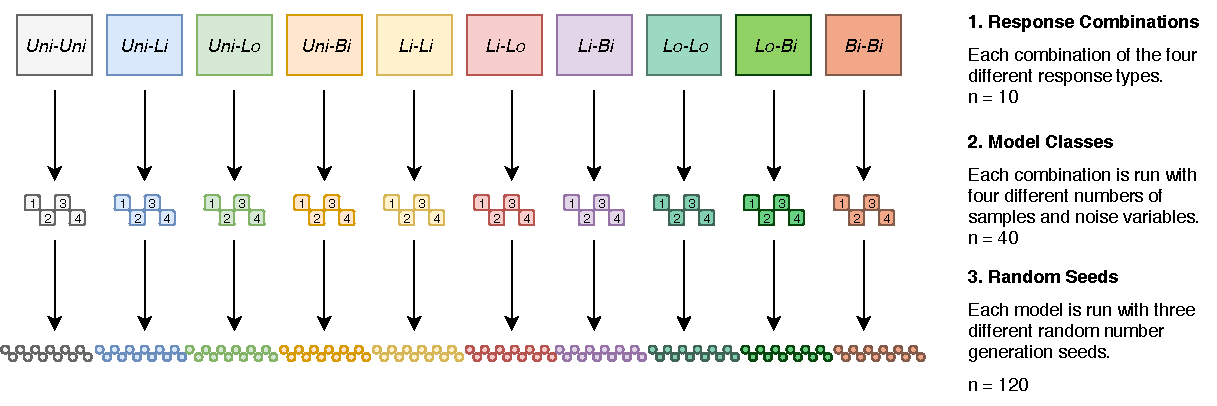
\includegraphics[width=1\linewidth]{../02_Figures/Flowchart}
			\caption{Flowchart of the simulation process. All possible combinations of the four response types unimodal (uni), linear (li), logistic (log) and bimodal (bi) were run in four different classes. The classes differed in how many samples are taken from the simulated community and in how many noise variables are included (see Table \ref{table:classes}).}
			\label{fig:flowchart_simulation}
		\end{figure}
	

		%------------------------------%
		%&	p-Werte 	
		%------------------------------%
		I used \textit{p}-values to compare the method's performances. While their use has been repeatedly criticized for over 50 years \citep[e.g.][]{rozeboom1960fallacy}, they provide a valuable means to compare methods as disparate as those tested herein. 
		%
		Three of the four methods (\textit{viz.} GLM$_{mv}$, db-RDA and CCA) provide \textit{p}-values for the influence of environmental variables on species abundances. Further, the use of \textit{p}-values in ecology and related fields is still wide spread \citep{FIDLER2006} and their performance is thus of practical importance. \\


	%------------------------------%
	%& GLM-MV
	%------------------------------%
	\subsection{Multivariate Generalized Linear Models}

		GLM$_{mv}$s are collections of $S$ separately fitted GLMs. 
		%
		Their likelihood ratios for each environmental variable are summed up to obtain the sum-of-Likelihood-Ratios statistic. 
		%
		This test statistic can provide a multivariate \textit{p}-value, showing whether an environmental variable has a statistically significant effect on the mean community abundance. 
		%
		By summing the likelihood ratios one assumes that species responses are independent of each other. 
		%
		This assumption is relaxed in the hypothesis tests because significance is assessed via row resampling, which preserves the correlation structure. 
		%
		Two alternative, computationally more demanding, test statistics are available: the Wald and the score test statistic. 
		%
		Both explicitly account for correlation between variables, by using Generalized Estimation Equations as proposed by \citet{Warton2011a}.\\ 
		%   
		The effect of each individual species can be assessed by the deviations of the univariate GLMs. 
		%
		Their \textit{p}-values are adjusted to multiple testing by controlling the family-wise type I error rate using a resampling-based version of the \textit{Holm's step-down multiple testing procedure} \citep{Westfall1993}. 
		%
		These adjusted \textit{p}-values tend to be very conservative \citep{Warton2018}. \\
		
		Each model was fit with negative binomial, Poisson, and normal residual distribution and their respective canonical links.
		%
		The fit of the three different models was checked with Dunn-Smith residual-plots and Akaike's Information Criterion \citep[AIC, ][]{akaike1974new}.
		%
		Hypothesis tests for the best fitting model were conducted using the likelihood ratio statistic, each model was resampled 500 times using the PIT-trap bootstrap procedure \citep{Warton2017}.
		%
		Besides resampling, no adjustment for inter-species correlations was used.\\

	%------------------------------%
	%& db-RDA
	%------------------------------%
	\subsection{Distance Based Redundancy Analysis}

		db-RDA  is the constrained form of Principal Coordinates Analysis (PCoA), an eigenvalue-based ordination conducted on distance matrices.
		%
		In a PCoA, $\mathbf{Y}$ is transformed into a centered distance matrix $\mathbf{D}$.
		% 
		Eigenvectors of $\mathbf{D}$, are scaled to the length of $\sqrt{\lambda_k}$, with $\lambda_k$ being the eigenvalue of the $k^{th}$ eigenvector $u_k$. 
		%
		The scaled eigenvectors are the columns of the principal coordinates matrix $\mathbf{PC}$ \citep{gower1966some}.
		% 
		The $\mathbf{PC}$ matrix is then used as a response matrix in an RDA. 
		%
		The db-RDA preserves the distance metric which was used to calculate $\mathbf{D}$, which can be metric, semi- or non-metric, setting	 the method apart from MANOVA \citep{anderson2001new} and transformation-based RDA \citep{Legendre2001}. 
		%
		However, semi- and non-metric distances can produce negative eigenvalues which entail complex ordination axes. 
		%
		These are problematic as they can not be interpreted in a meaningful way. 
		%
		Adding a constant to the squared dissimilarities can correct this \citep[\textit{Lingoes correction}, ][]{gower1986metric}.
		%
		Hypothesis tests on the significance of individual constrained axes and environmental variables can be conducted using a pseudo-F-Statistic with permuted residuals  \citep{Legendre2011}.
		  	
		The semi-metric percentage difference distance metric was used. 
		%
		It was introduced by \citet{odum1950bird} and is commonly referred to as Bray-Curtis Distance \citep{Legendre2012}.
		%
		It is asymmetric and thus avoids the double zero problem  \citep{Legendre2012} and is generally acknowledged to have desirable properties for species abundance data \citep{bloom1981similarity,faith1987compositional}.
		%
		Hypothesis tests on axes and covariables were conducted with 999 permutations. 

	
	%------------------------------%
	%&  CCA
	%------------------------------%
	\subsection{Canonical Correspondence Analysis} \label{subsec:CCA}
	
		CCA has long been the most common way to estimate the parameters of a CGO, even though it is only an approximation of the maximum likelihood solution. 
		%
		It assumes equal tolerances, equal maximal abundances, uniform distribution of species optima and site scores over the latent variable space and bell-shaped responses \citep{TerBraak1986}. 
		%
		The assumptions are collectively known as the \textit{species packing model}. 
		%
		\citet{Palmer1993}, \citet{Johnson1999} and \citet{Zuur1999} confirmed the validity of the approximation and its robustness towards violations against assumptions of the species packing model in simulation studies.
		%
		Nonetheless, the restrictive assumptions were widely criticized \citep[e.g.][]{Austin1994}. \\
		%
		An iterative algorithm is used to obtain estimates. First, arbitrary values are assigned to the site scores (positions of sites in latent variable space, $\mathbf{Z}$). 
		%
		These are used to calculate the species optima  $u$ (henceforth species scores) as in Eqn. \ref{eq:CCA_species_scores}.
		%
		\begin{equation}\label{eq:CCA_species_scores}
		\mathbf{u} = \mathbf{D}_c \mathbf{Y}^t \mathbf {Z}
		\end{equation}
		%
		Where $\mathbf{u} = (u_1\ ...\ u_S)^t$, $\mathbf{D}_c$ is a diagonal matrix with the abundance of species $s$ across all sites as its $s,s^{th}$ element and $\mathbf{Y}^t$ denotes the transpose of $\mathbf{Y}$.\\
		%
		The species scores are in turn used to calculate the site scores as their weighted average $\mathbf{Z}_{wa}$ (Eqn. \ref{eq:CCA_site_scores}) 
		%
		\begin{equation} \label{eq:CCA_site_scores}
			\mathbf{Z}_{wa} = \mathbf{D}_r^{-1} \mathbf{Y} \mathbf {u}
		\end{equation}
		%
		where $\mathbf{D}_r$ is a diagonal matrix with the abundance of all species at site $n$ as its $n,n^{th}$ element and $\mathbf{D}_r^{-1}$ denotes the inverse of $\mathbf{D}_r$. 
		%
		$\mathbf{Z}_{wa}$ is regressed against $\mathbf{X}$ to obtain the weighted regression coefficient $\alpha$. 
		%
		\begin{equation}\label{CCA_canocical_weights}
		\alpha = (\mathbf{X}^t \mathbf{D}_r \mathbf{X})^{-1} \mathbf{X}^t \mathbf{D}_r \mathbf{Z}_{wa}
		\end{equation}
		%
		Lastly, $\mathbf{Z}$ is calculated as the product of $\mathbf{X}$ and $\mathbf{\alpha}$. 
		%
		This procedure is repeated until convergence. \\
	    
		The distance between sites (scaling 1) or species (scaling 2) in CCA approximates their two dimensional $\chi^2$-distance, i.e. the Euclidean distance between the expected abundances under the null hypothesis, that abundances do not change along environmental gradients, and the actual data.
		%
		The absolute difference between expectation and measurement is known as \textit{total inertia}. 
		%
		The ratio of constrained inertia, i.e. variation that can be explained by constrained axes, and total inertia is a general measure of fit for a CCA.
		%
		The chi-squared-distance is asymmetrical and therefore is unaffected by the double zero problem, but it has been criticized since the same absolute change in a rare species is weighted much stronger than an equal change in an abundant species \citep{greig1983quantitative}. 
		%
		The relation between ecological and chi-squared distance is weaker than in other metrics \citep{faith1987compositional,Legendre2001}.
		%
		The significance tests for axes or environmental variables are calculated using a pseudo-F-Statistic as in db-RDA.
	
	%------------------------------%
	%&  CAO/CQO
	%------------------------------%
	\subsection{Constrained Additive and Quadratic Ordination}

		CQO and CAO are based on VGLMs and their additive counterpart VGAMs, respectively. 
		%
		VGLMs expand GLMs, in that they can encompass multiple response variables, each with a separate linear predictor. 
		%
		The modeled responses can be other parameters than the mean(e.g. the variance) and
		%
		VGLMs are not restricted to residual distributions from the exponential family. \\
		%CAO and CQO are based on vector generalized models. The basic VGLM is given in Eqn. \ref{eq:VGLMbasic}.
		%\begin{equation}\label{eq:VGLMbasic} \tag{2.2.1}
		%\eta_s(\mathbf{x}) = g_s(\theta_s) = \sum_{k = 1}^M \beta_{(s)k}\ x_k  	
		%\end{equation}
		%Where $\eta_s$ is the linear predictor for the $s^{th}$ response variable, $g_s$ is the parameter link function for the parameter $\theta_s$ and $\beta_{(j)k}$ is the regression coefficient for response variable $s$ and covariable $k$.\\
		
		Both methods employ \textit{Reduced Rank VGLMs/ VGAMs} (RR-VGLM/ VGAM). 
		%
		In RR-VGLMs the $M$ environmental variables are reduced to $R$ latent variables $\nu$. 
		%
		Therefore, the design matrix $\mathbf{X}$ and hat matrix $\mathbf{B}$ are each partitioned into two subsets 
		$\mathbf{X} = (\mathbf{x}_1^T,\mathbf{x}_2^T)^T$; $\mathbf{B} = (\mathbf{B}_1^T,\mathbf{B}_2^T)$. 
		%
		$\mathbf{x}_1$ and $\mathbf{B}_1$ contain covariables and corresponding regression coefficients, which do not contribute to the latent variables. 
		%
		In practice, $\mathbf{x}_1$ often only contains the intercept and $\mathbf{B}_1$ is thus a vector of 1s with length $M$. $\mathbf{B}_2$ is reduced to a rank $R$ matrix (with full column rank). 
		%
		This is done by reduced rank regression \citep{Anderson1951, izenman1975reduced}, which determines a low-rank matrix that is an optimal
		approximation of a full rank matrix. 
		%
		Unlike in db-RDA or CCA, the researcher specifies the number of latent variables, i.e. the rank of $\mathbf{B}_2$, \textit{a priori}.
		%
		It is referred to as the rank of the method. \\
		%
		The low-rank matrix $\mathbf{B}_2$ is decomposed into two thin matrices $\mathbf{A}$ and $\mathbf{C}$ (see Eqn. \ref{eq:ReduceB2}).
		
		\begin{equation}\label{eq:ReduceB2}
		\mathbf{B}_2^T = \mathbf{A}\ \mathbf{C}^T	
		\end{equation}
		
		The matrix $\mathbf{C}^T$ contains the constrained coefficients, which act as constants in the linear combination of $\mathbf{x}_2$ that constitutes the latent variables. (cf. Eqn.\ref{eq:ctx2})
		
		\begin{equation}\label{eq:ctx2}
		\mathbf{\nu} = \mathbf{C}^T \mathbf{x}_2	
		\end{equation}
		
		The linear predictor therefore becomes:
		
		\begin{equation}\label{eq:ctx3}
		\eta = \mathbf{B}_1^T \mathbf{x}_1 + \mathbf{A} \mathbf{\nu}	
		\end{equation}
		
		
		CQO is an adaption of RR-VGLMs to ecological data sets.
		%
		It assumes that the response variables show symmetric and bell-shaped responses to the underlying gradients represented by the latent variables.
		%
		To this end, quadratic RR-VGLM of the kind of Eqn. \ref{eq:CQO1} are used.
		
		\begin{equation}\label{eq:CQO1} 
		\eta_s = \beta_{(s)1} x_{(s)1} + \beta_{(s)2} \nu + \beta_{(s)3} \nu^2	
		\end{equation} 
		
		The response curve is unimodal for all $\beta_3 < 0$.
		%
		CQO does not assume the species packing model of the CCA.
		%
		Three different assumptions can be made concerning the tolerances: (i) equal tolerances, (ii) unequal tolerances and (iii) identity tolerances.
		% 
		The equal tolerance assumption expects tolerance matrices $\mathbf{T}$ to be equal for all species $\mathbf{T}_1 = \mathbf{T}_2 = ... = \mathbf{T}_S$.
		%
		With the unequal tolerances assumption, the tolerance for each species is estimated separately.
		% 
		For one species $T_s \equiv I_R$, as long as any species has a positive-definite tolerance matrix. 
		%
		Lastly, identity tolerance sets $T_s \equiv I_R$ for all species. 
		%
		This implies the equal tolerance assumption.  
		% 
		Equal or identity tolerance models are expected to be faster and easier to interpret but unequal tolerance models should fit the data better \citep{yee2015vector}.\\
		% 
		In a CAO the assumptions of symmetric bell shaped responses is relaxed by using a smooth function for $\nu$. 
		%
		The RR-VGAM can be conceptualized as fitting a generalized additive model for each species against the latent variables.
		%
		As of now, the method is still limited in its capabilities \citep{Yee2006}.
		%
		Only rank-1 models can be fitted and only to Poisson or binary responses.  
		%
		\citet{Yee2006} advocates to use CAO for exploratory data analysis and CQO for inference, akin to using Generalized Additive Models as a diagnostic tool before running GLMs \citep{Hastie2008}.\\
		  
		 
		CAO and CQO were run with Poisson residual distribution and the canonical log-link function.
		%
		The effective nonlinear degrees  of freedom was set to 1.5 as suggested by \citet{yee2015vector}.
		%
		Constrained coefficients on the first axis were restricted to be positive. 
		%
		Each model was run ten times and the solution with the lowest deviance was used to safeguard against local solutions.
		% 
		% General Info - absolute values 
		For the calculation of mean values and standard deviations the constrained coefficients of CAO and CQO were transformed to absolute values. 
		%
		To asses the influence of environmental variables on the latent variable, the algebraic sign is not of interest, since it only shows the directionality of the former on the latter.
		%
		Rank-1 models were run for CAO, rank-1 and rank-2 models with all three tolerance settings for CQO. 
		%
		The optimal number of ranks was found to be two for all models, determined by the AIC as proposed by \citet{yee2003reduced}. \\
		
		
	\subsection{Software}
		All simulations and analyses were done in R 3.4.4 \citep{RCT2018}.
		%
		GLM$_{mv}$s were conducted with mvabund 3.13.1. \citep{Wang2018}, db-RDA and CCA with vegan 2.5-2 \citep{Oksanen2018} and CAO/CQO with VGAM 1.0-5 \citep{Yee2018}. 
		%
		R-scripts for the simulations as well as the analyses are available on \href{https://github.com/JonJup/Master-Thesis.git} {GitHub}.


